\chapter{Interpretation der Ergebnisse (VR)}

\section{Höhenruder Trimmkurve}

Aus den aufgezeichneten Daten lässt sich ein linearer Zusammenhang zwischen dem Anstellwinkel alpha und dem 
Höhenruderausschlag $\eta$ feststellen. Mit steigendem Höhenruderausschlag sinkt der Anstellwinkel. 
Der Anstellwinkel $\alpha$ beschreibt den Winkel zwischen dem Fluggeschwindigkeitsvektor und der Flugzeuglängsachse. Ein positiver Winkel $\alpha$ bedeutet, dass die Flugzeuglängsachse positiv gegenüber dem Fluggeschwindigkeitsvektor gedreht ist. 

%\begin{figure}[h]
%		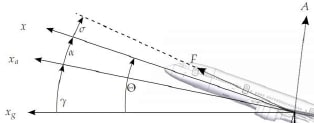
\includegraphics{./Bilder/Anstellwinkel_Definition.jpg}
%	\caption{Definition Anstellwinkel}
%	\label{alpha_def}
%\end{figure}
%\begin{figure}
%	\includegraphics{./Bilder/Höhenruderausschlag_Definition.jpg}
%	\caption{Definition Höhenruderausschlag}
%	\label{fig:eta_def}
%\end{figure}


Der Winkel des Höhenruders $\eta$ beschreibt die Auslenkung des Ruders gegenüber einer Neutrallage. Ein negativer 
Höhenruderausschlag bedeutet eine lokale Absenkung des Auftriebs am Höhenleitwerk, sodass es zum Absinken des Hecks kommt (Nose-up). In die positive Richtung ausgeschlagen steigt der Auftrieb am Höhenleitwerk, sodass sich das Heck hebt (Nosedown). 
Damit decken sich die Messdaten der Do 28 zu Anstellwinkel und Höhenruderausschlag mit der Theorie.




\section{Auftriebsbeiwert über Anstellwinkel}

Der Auftriebsbeiwert $C_A$ steigt linear mit zunehmendem Anstellwinkel alpha. $C_{A0}$ bezeichnet den Auftriebsbeiwert bei einem Anstellwinkel von null. $\alpha_0$ beschreibt den Nullauftriebswinkel, an dem der Auftriebsbeiwert null annimmt, das heißt kein Auftrieb mehr generiert wird. Der Auftriebsanstieg $C_{A\alpha}$ berechnet sich wie folgt:

\begin{equation}
C_{A\alpha}=\frac{dC_A}{\alpha}
\end{equation}

	
Bei der Anströmung eines Tragflügels wird die Luft umgelenkt und es entsteht eine Druckdifferenz zwischen Tragflügelober- und Oberseite, was als Voraussetzung für die Entstehung von Auftrieb ist. Der Anstellwinkel des Flügels ist dabei der größte Einflussfaktor für den Auftriebsbeiwert. Für kleine Winkel $\alpha$ mit anliegender Strömung gilt daher der lineare Zusammenhang

%\[\(C_a\)=\(C_a\alpha\)(\alpha-\(alpha_0\))\] \\

Damit stimmen die Messdaten mit der Theorie überein. Jedoch lassen sich keine Aussagen über den maximalen Auftriebsbeiwert treffen, da die aufgenommenen Anstellwinkel im Bereich der anliegenden Strömung liegen und der höchste Auftriebsbeiwert erst kurz vor dem Abreißen der Strömung erreicht wird. 

Die für $C_A$ und $C_W$ errechneten Werte werden für die Erstellung der Lilienthalpolare gegeneinander aufgetragen und mit einer quadratischen Regression angenähert. Daraus ergibt sich für den Nullwiderstand $C_{W0}$ ein Wert von 0,0503, für den Polynomterm erster Ordnung ein Koeffizient von 0,0033 und für den zweiten Grades ein Koeffizient von 0,0258. 
Aus der Lillienthal-Polare lässt sich die minimale reziproke Gleitzahl ermitteln, die die Höhendifferenz beim Sinken des Flugzeugs bei einer bestimmten Flugstrecke beschreibt. Zur Ermittlung der minimalen reziproken Gleitzahl wird eine Tangente durch den Ursprung an die entstandene Polare gelegt. Am Schnittpunkt der Tangente mit der Polaren können die zugehörigen Beiwerte $C_A^*=$1,39 und  $C_W^*$=0,105 abgelesen werden, mit denen die reziproke Steigung der Tangente mit

%\[ \(\epsilon_min\)=  \(C^{*}_W\) \div \(C^{*}_A\)=0,105 \div 1,39=0,0755\] \\

berechnet werden kann. Der Gleitwinkel $\gamma$, der die Drehung des Geschwindigkeitsvektor gegenüber der geodätischen Horizontalebene in x-Richtung beschreibt, ergibt sich zu

%\[\gamma=\arctan(- (\(C^{*}_W\) \div \(C\{*}_)^A\])) = arctan(-(0,105 \div 1,39)) = -4,32~�\]  \\

Aus den bekannten Werten $C_{W0}$ und $C^{*}_A$ lässt sich der Widerstandsanstieg k wie folgt berechnen: 

%\[k= \(C_W0\) \div  \(C^{*} _A\)^{2}=0,0451 \div 1,39^{2}=0,2334 \] \\

 In der Theorie wird an dieser Stelle ein positiver Wert für k erwartet, was bedeutet, dass die aus der Regression entnommenen Werte falsch sind. Da nur vier verschiedene Flugzustände aufgenommen werden konnten, ist die Regression außerhalb des Messwertbereichs ungenau. 

\section{Widerstand über Fluggeschwindigkeit}
tbd

\section{Staudruck über Anstellwinkel}
tbd

\section{Fluggeschwindigkeit über Anstellwinkel}
tbd
